\section{Generating synthetic pandemics}



To be able to compare the performances of the models, one need pandemic data to compare them. 
As the objective was to obtain the most consistent results, I decided not to train and compare the models on real data as this data is limited and biaised: the results would not have been relevant when facing a new pandemic. 
All the simulations in this paper are made on a fixed population of $10^6$ agents. 

\subsection{Covasim}

To generate the pandemics,  Covasim \cite{kerr2021covasim}, a python library that can simulate the evolution of a pandemic, was used. 
Covasim is an agent-based model that can simulate the spread of a pandemic in a population. 
This model takes as an input many parameters such as the population type, the population size, the age repartition... and outputs a complete description of the pandemic, with real-time values of each relevant piece of information, such as the number of severe, of asymptomatic... but also physical values such as the value of the reproduction number. 
Covasim enables to generate a huge diversity of pandemics, thanks to the plurality of parameters that can be given as input to the model, but also with interventions that can be planned by the users. 
These interventions can help to assess the impact of a vaccination campaign, or lockdown scenarios. 
They represent relatives changes in the probabilities of transmission. 
Covasim was used by policymakers during the Covid 19 outbreak to adapt their strategies of mitigation, for instance in Australia,Vietnam, India and United States (\cite{kerr2021covasim}). 

\subsection{First pandemics}

For the implementation and the first tests of the models, two pandemics were generated. 
The first one focusing on the new deaths count and the second one focusing on the number of hospitalized count. 
I quickly decided to move to the second pandemic, as the variable 'new deaths' is neither relevant nor continuous (which caused problems in the implementation of some models, namely SIRH models).


The different interventions were based on mobility reports from Västtrafik (see appendix \ref{sec:appendix}), the public transport company of the city of Gothenburg. 
They were reported during the Covid 19 pandemic and have been retrieved in \cite{gerlee2021predicting}.
These interventions correspond to 53 relative weekly variations of the mobility, with a reference value of 1 for the first week of the report, which correspond to the 9-th week of 2020. 


\subsection{Generating diverse pandemics}
\label{sec:generating_divserse_pandemics}
In order to evaluate the performances of my models on a wide range of pandemics, a training set of pandemics was generated. 
A huge diversity of pandemics is needed to determine the most consistent model.
It is so relevant to identify the key parameters that generate this diversity.
As Covasim has a very huge set of inputs parameters, a first subset of key parameters was identified: the spread parameters and the severity parameters. 
The severity parameters are the 4 parameters that correspond to the probability for an agent to get from a compartment to another (for instance from infected to crictical). 
The spread parameters are 9 parameters that represent the distribution of probability of the time spend by an agent in a compartment (such as infected, crictical...) once he entered it. 
This set of 13 parameters is then noted as $S$. 
This distribution is a log-normal distribution, but the spread-parameters correspond to the mean of this log-normal distribution
All the parameters have a default value of 1, which corresponds to keeping the reference value. 
I decided to select 4 parameters and to make them vary in $[0.5, 1, 2]$, leading to a set of 81 pandemics. 
To select the 4 parameters that generated the most diversity, different diversity metrics were computed. 

Let $Y_1$ ,  $Y_2 \in \mathbb{R}^n$  be two time series of $n$ days representing the number of hospitalized in two pandemics, and $Y'$ and $Y''$ the first and second derivatives of $Y$.  \\[0.2cm]

Let :  \\

$
\begin{aligned}
    &\mathcal{L}_1(Y_1, Y_2) = \| Y_1 - Y_2 \|_{L_1}  \\
    &\mathcal{L}_2(Y_1, Y_2) = \| (\frac{max(Y_1)}{max(Y_2)} ;\frac{max(Y_1')}{max(Y_2')} ; \frac{max(Y_1'')}{max(Y_2'')} , \| \tilde{Y_1} - \tilde{Y_2} \|_{L_1}, \| \tilde{Y_1'} - \tilde{Y_2'} \|_{L_1} , \| \tilde{Y_1''} - \tilde{Y_2''} \|_{L_1}) \|_{L_2} \\
    &\mathcal{L}_3 = \mathcal{W}(\tilde{Y_1} - \tilde{Y_2}) \text{, with }\mathcal{W} \text{ the Wasserstein distance.} \\
    &\mathcal{L}_4(Y_1, Y_2) = \| (\frac{max(Y_1)}{max(Y_2)} ;\frac{max(Y_1')}{max(Y_2')} ; \frac{max(Y_1'')}{max(Y_2'')} , \mathcal{W} (\tilde{Y_1} - \tilde{Y_2}),\mathcal{W} (\tilde{Y_1'} - \tilde{Y_2'}) , \mathcal{W} (\tilde{Y_1''} - \tilde{Y_2''})) \|_{L_2} \\
\end{aligned}
$


To determine which measure to use, I generated 14 pandemics. 
Each pandemic but the last one has default parameters except one of them which was doubled. 
The last pandemic has only default parameters. 

For each norm $\mathcal{L}_k$, I determined $s$,  the subset of 4 pandemics that maximized the following quantity:\\

\[ \mathcal{L}_k(S) = \sum_{i, j \in s, i \neq j} \mathcal{L}_k(Y_i, Y_j) \]

\begin{figure}
    \centering
    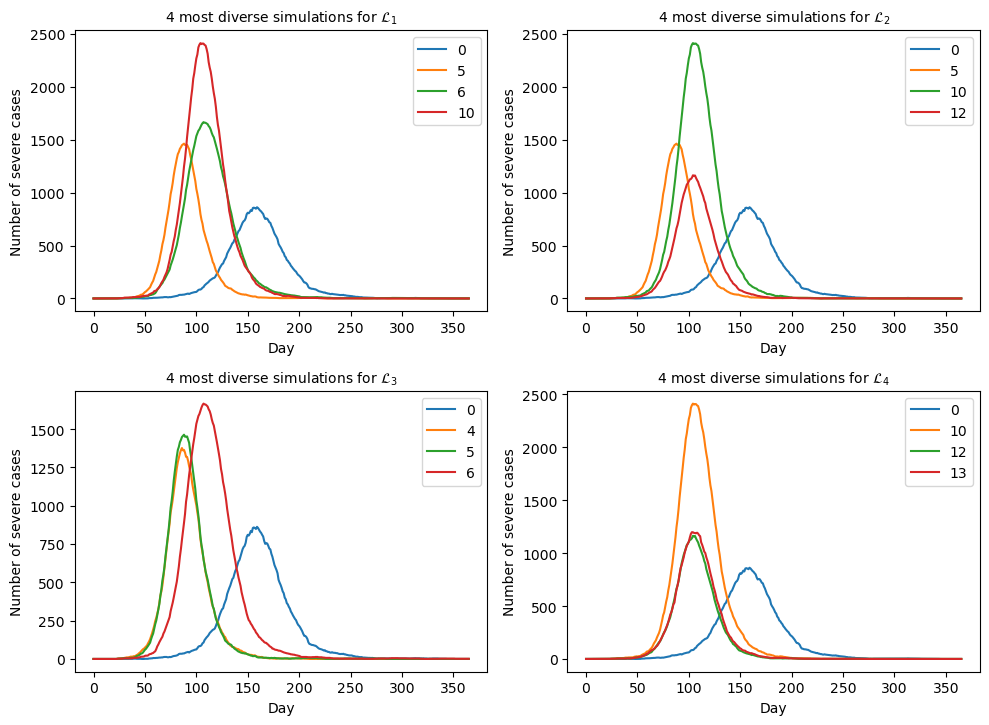
\includegraphics[width=0.8\textwidth]{figures/most_different_pandemics.png}
    \caption{4 most diverse pandemics according to each norm.}
    \label{fig:diversity_pandemics}
\end{figure}


The 4 most diverse pandemics (in the subset of 14 pandemics generated) according to each norm are shown in the Fig.\ref{fig:diversity_pandemics}.
As "diversity" is not countable, a human choice was necessary to choose the most relevant norm.
According to Fig. \ref{fig:diversity_pandemics}, I decided to select $\mathcal{L}_2$.
But, keeping the parameters \texttt{[0, 5, 10, 12]} would not be accurate, as the parameters were changed independently, and the diversity did not take into account the correlation between some of them. \\

Finding the parameters that maximise the $\mathcal{L}_2$ diversity is equivalent to solve the following problem : \\

$ s_{opt} = \underset{s \subset S , \vert s \vert =4 }{argmax  } \mathcal{ L}(s)$, with $ \mathcal{L}(s)= \sum_{p_1, p_2 \in \mathcal{P}_g(s)  }{\mathcal{L}_2(p_1,p_2)}$, and  $\mathcal{P}_{g}(s)$ the set of the 81 pandemics generated with the 4 parameters of $s$.

However, generating a pandemic with \texttt{Covasim} is time consuming, and it is not possible to compute the diversity of each set of 4 parameters $s$ included in $S$ (the set of all 13 parameters).\\[1cm]


A MCMC algorithm \cite*{diaconis2009markov} was then implemented, to perform a clever grid search on the different subsets $s \subset S $ of parameters.
The MCMC algorithm is a method which is used to sample from a distribution that can't be directly sampled. 
The main idea is to construct a Markov Chain whose stationary distribution is the objective distribution.

Let $\mathcal{S} = \{ s\subset S ;  \vert s \vert = 4 \}$ be the support of the target distribution, which is, in our case, the set of all the 715 combinations of the 4 parameters among the 13 different possible, and let $\pi$ be the target distribution on $\mathcal{S}$.
$\forall s \in \mathcal{S}, \pi(s) = \frac{\mathcal{L}(s)}{\sum_{s \in \mathcal{S}}  \mathcal{L}(s)} $. $\pi$ is not directly computable as it is too time consuming to compute the denominator.
We suppose that $\forall s \in \mathcal{S}, \mathcal{L}(s) >0$.
It is a reasonable assumption, as $\mathcal{L}(s) = 0 $ means that the 81 pandemics generated   are strictly identical. 

For each $s = [a, b, c, d] \in \mathcal{S}$, let $ne(s)$ be the set of the neighbours of $s$, i.e the set of all the elements of $\mathcal{S}$ who have only one parameter different from $s$. 
For instance, $[0, 3, 9, 12] \in ne([0, 3, 10, 12])$, but $[0, 3, 9, 12] \notin ne([0, 3, 8, 10])$.\\

Let $U_n$ be a sequence of independent uniform random variables on $[0, 1]$ and $\forall s \in \mathcal{S}$, let $U_{n}^{ne(s)}$ be a sequence of independent uniform random variables on $ne(s)$ .
Let $s_0 \in \mathcal{S}$ and let  $S_n$ be the random sequence defined as follow : \\


\[
 \left\{
    \begin{aligned}
        & S_0 = s_0 \\
        & \forall n \in \mathbb{N}, \alpha_n = \frac{\mathcal{L}(U_{n}^{ne(S_n)})}{\mathcal{L}(S_n)} \\
        & \forall n \in \mathbb{N}, S_{n+1} = U_{n}^{ne(S_n)} \mathbb{1}_{\{U_n < \alpha_n\}} + S_n \mathbb{1}_{\{U_n > \alpha_n\}}
\end{aligned}
\right.
\]
\\[0.5cm]

This formula means that at each iteration, a neighbourgh of $S_n$ is uniformly selected among all the neighbours of $S_n$ (it is $U_n^{ne(S_n)}$). 
The Markov Chain moves to this neighbourgh if the value of  $\mathcal{L}(U_n^{ne(S_n)})$ is higher than the value of the function $\mathcal{L}(S_n)$ at the current state.
If the new value of $\mathcal{L}$ is smaller, the Markov Chain moves with a probability that is equal to the ratio of the two values.
This way of moving on the different subsets prevents to be stucked in a local maxima but avoids exploring dummies areas, in which the diversity is very small. \\
As $S_{n+1}$ is a function of $S_n$ and of other independent random variables, the sequence $S_n$ is a homogenous Markov Chain.

The transition matrix of this Markov Chain is the following: 
\[
K(s, s'): \left\{
\begin{aligned}
& 0 \text{ if } s' \notin ne(s) \text{ and } s' \neq s   \\
& \frac{1}{Card(ne(s))} = \frac{1}{36} \text{ if } s' \in ne(s) \text{ and } \frac{\mathcal{L}(s')}{\mathcal{L}(s)} > 1 \text{ and } s' \neq s \\
& \frac{1}{36} \times \frac{\mathcal{L}(s')}{\mathcal{L}(s)} \text{ if } s' \in ne(s) \text{ and } \frac{\mathcal{L}(s')}{\mathcal{L}(s)} \leq 1  \text{ and } s' \neq s  \\
& 1 - \sum_{s' \in \mathcal{S}, s' \neq s}K(s, s') \text{ if } s' = s 
\end{aligned}
\right.
\]
\\[0.3cm]

Let $(s, s') \in \mathcal{S}^2$. Let us suppose that $ s' \neq s$, that  $s' \in ne(s)$, and that $\mathcal{L}(s) < \mathcal{L}(s')$ (the other case is symmetric). \\[0.15cm]
$
\begin{aligned}
    \pi(s)K(s, s') &=  \frac{\mathcal{L}(s)}{\sum_{s \in \mathcal{S}} \mathcal{L}(s)} \times \frac{1}{36} \quad \text{as} \ \mathcal{L}(s) < \mathcal{L}(s') \\
    &=  \frac{\mathcal{L}(s)}{\sum_{s \in \mathcal{S}} \mathcal{L}(s)} \times \frac{1}{36} \times \frac{\mathcal{L}(s')}{\mathcal{L}(s')} \\
    &=  \frac{\mathcal{L}(s')}{\sum_{s \in \mathcal{S}} \mathcal{L}(s)} \times \frac{1}{36} \times \frac{\mathcal{L}(s)}{\mathcal{L}(s')} \\
    &= \pi(s')K(s', s)\\[0.3cm]
\end{aligned}
$
\newline
Indeed, each subset $s$ has 36 neighbourgh, as there are 13 parameters and one can replace each parameter of $s$ by any of the 9 others. \\

If $s' \notin ne(s)$, then $s \notin ne(s')$ and $K(s, s') = 0$.
We directly have $\pi(s)K(s, s') = 0 = \pi(s')K(s', s)$.\\

Thus, $\pi$ is \textbf{reversible} for $K$.\\[0.3cm]
Let $(s, s') \in \mathcal{S}^2$. Let us note $(a, b, c, d)$ and $(a', b', c', d')$ the elements of $s$ and $s'$.
We note : \\
$s_1 = [a', b, c, d]$\\
$ s_2 = [a', b', c, d]$ \\
$s_3 = [a', b', c', d]$ \\


$
\begin{aligned}
    \mathbb{P}(S_{n+4}=s'\vert S_n = s) & \geqslant \mathbb{P}(S_{n+4} = s' \cap  S_{n+3}= s_3 \cap S_{n+2} = s_2 \cap S_{n+1} = s_1 \vert S_n = s) \\
    & \geqslant \mathbb{P}(S_{n+4} = s' \vert S_{n+3} = s_3 \cap S_{n+2} = s_2 \cap S_{n+1} = s_1 \cap S_n = s) \\
    & \quad\quad\quad\quad \times \mathbb{P}(S_{n+3} = s_3 \cap S_{n+2} = s_2 \cap S_{n+1} = s_1 \vert S_n = s) \text{  (Baye' s Formula)}\\
    & \geqslant \mathbb{P}(S_{n+4} = s' \vert S_{n+3} = s_3)\\
    & \quad\quad\quad\quad  \times \mathbb{P}(S_{n+3} = s_3 \cap S_{n+2} = s_2 \cap S_{n+1} = s_1 \vert S_n = s)  \text{ (by Markov's property)}\\
    & \vdots \\
    & \geqslant \mathbb{P}(S_{n+4} = s' \vert S_{n+3} = s_3) \times \mathbb{P}(S_{n+3} = s_3 \vert S_{n+2} = s_2) \times \mathbb{P}(S_{n+2} = s_2 \vert S_{n+1} = s_1) \\
    & \quad\quad\quad\quad \times \mathbb{P}(S_{n+1} = s_1 \vert S_n = s) \text{ (by Markov's property)}\\
    & \geqslant (\frac{1}{36})^4 \times min (1, \frac{\mathcal{L}(s')}{\mathcal{L}(s)}) \times min (1, \frac{\mathcal{L}(s_3)}{\mathcal{L}(s_2)}) \times min (1, \frac{\mathcal{L}(s_2)}{\mathcal{L}(s_1)}) \times min (1, \frac{\mathcal{L}(s_1)}{\mathcal{L}(s)})  \\
    & > 0 \\
\end{aligned}
$

Thus, $S_n$ is \textbf{irreducible}.\\

A Markov chain of transition matrix $P$ on the support $\mathcal{S}$ is said to be \textit{aperiodic} if: \\
$\forall s \in \mathcal{S}, \forall s' \in \mathcal{S}, \exists N \in \mathbb{N}, \text{ s.t } \forall n > N, P(s, s')^n >0 $ \cite{bodineau2015modelisation}\\

First, note that $\forall s \in \mathcal{S}$,  $s$ is a local minimum (i.e if $\forall s' \in ne(s), \mathcal{L}(s') > \mathcal{L}(s) $) if and only if $K(s,s)=0$\\

Thus, if $s$ is not a local minimum, then $K(s, s)>0$. Moreover, $ \forall s \in \mathcal{S}, \forall s' \in ne(s)$, if $s\neq s'$, then $K(s, s') \neq 0 $\\[0.3cm]
Let $(s, s')  \in \mathcal{S}^2$. \\

\begin{itemize}
    \item If $s'$ is not a local minimum, \\
     $\forall n >4, \mathbb{P}(S_{n} = s' \vert S_0 = s) \geqslant \mathbb{P}(S_{4} = s' \vert S_0 = s) \times K(s', s')^{n-4} > 0 $ \\
    \item If $s'$ is a local minimum,  $\forall s^* \in ne(s')$, $s^*$ is not a local minimum and $K(s^*, s^*) \neq 0$. \\
    $\forall n>5$, $\mathbb{P}(S_n = s' \vert S_0 = s)   \geqslant \mathbb{P}(S_3=s^* \vert S_0 = s) \times K(s^*, s^*)^{n-4} \times K(s^*, s') >0 $\\
    
\end{itemize}

Thus $S_n$ is an \textbf{aperiodic} Markov Chain.\\


Finally, according to the \textbf{Theorem 5.5 } from \cite*{bodineau2015modelisation}, as $S_n$ is irreducible and aperiodic, as $\pi$ is the stationary distribution, and as $\mathcal{S}$ is countable, $S_n$ converges in distribution to $\pi$.\\


The most probable set that will be sampled by $S_n$ is the one that maximises the diversity.
I implemented this MCMC algorithm to maximise $\mathcal{L}_2$ on $\mathcal{S}$ . 
The first value of the sequence was a clever starting point: the four parameters that maximized $\mathcal{L}_2$ on the 14 pandemics generated earlier (Fig.\ref{fig:diversity_pandemics}).  
After 200 iterations, the set of parameters that maximised the diversity was \texttt{[2, 4, 9, 10] }, which correspond to the parameters \texttt{[sym2sev, asym2rec, rel\_symp\_prob, rel\_severe\_prob]}. 
They correspond respectively to the mean of the log-normal distribution representing the time spent in the compartment 'symptomatic' before moving into the compartment 'severe', the mean of the log-normal distribution representing the time spent in the compartment 'asymptomatic' before moving into the compartment 'recovered', to the scale factor for proportion of symptomatic cases and to the scale factor for proportion of symptomatic cases that become severe. (see \cite{kerr2021covasim}). 
The $\mathcal{L}_2$- diversity increased from 62353 to 93553. \\

To create the most diverse set possible, I used 4 different mobilities reports (Fig.\ref{fig:mobilities}), corresponding to constant mobility, annual variations, lockdown scenario and the reports from Vasträffik from \cite{gerlee2021predicting}. 
\begin{figure}
    \centering
    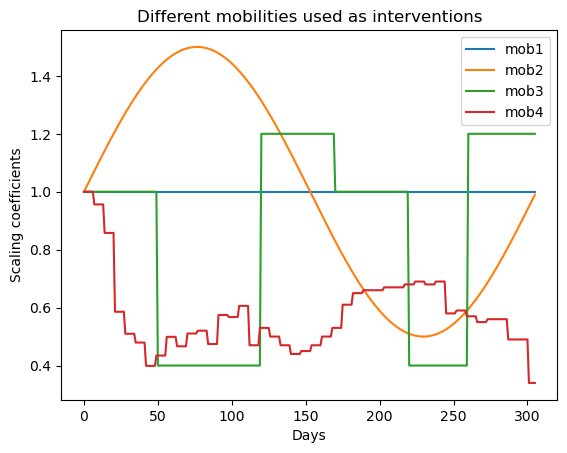
\includegraphics[width=0.5\textwidth]{figures/mobilities.png}
    \caption{Mobility reports.}
    \label{fig:mobilities}
\end{figure}
These time-varying mobilities enabled us to model more complex behaviours of the pandemics. 
I finally modelled 324 pandemics. 
Indeed each of the 4 parameters was scaled among 3 values : \texttt{[0.5, 1, 2]} and the 4 mobilities reports were used.

